\documentclass[11pt]{article}

% =========================
% Packages
% =========================
\usepackage[margin=1in]{geometry}
\usepackage{setspace}
\usepackage{booktabs}
\usepackage{longtable}
\usepackage{array}
\usepackage{amsmath}
\usepackage{amssymb}
\usepackage{amsthm}
\usepackage{hyperref}
\usepackage{tikz}
\usetikzlibrary{positioning,arrows.meta}
\usepackage{graphicx}
\usepackage{placeins}

\hypersetup{
  colorlinks=true,
  linkcolor=black,
  urlcolor=blue,
  citecolor=black
}

\setlength{\parskip}{0.6em}
\setlength{\parindent}{0pt}
\onehalfspacing

% =========================
% Document
% =========================
\begin{document}

\begin{center}
{\LARGE \textbf{The Dickinson Climate Classification}}\\
\vspace{0.25em}
{\large Caleb Dickinson}
\end{center}

% ============================================================
\section*{Abstract}

We introduce the Dickinson Climate Classification, a thermodynamically grounded, species-independent framework for classifying past, present, future, and hypothetical climates. The system explicitly separates thermal constraints from hydrological constraints, restricts aridity classification to climates that are neither polar, subpolar, nor alpine, and defines all classification boundaries using evenly spaced physical thresholds. Importantly, the system does not attempt to define the absolute limits of life; instead, it partitions climate space into analytically useful categories for comparative and predictive analysis across Earth’s paleoclimates, present climates, projected future warming scenarios, and ecologically relevant climatic states that may never occur on Earth.

\section*{Introduction}

The Dickinson Climate Classification differs fundamentally in both purpose
and structure from widely used systems such as Köppen and the UNEP aridity
index. The Köppen system is explicitly ecological and biogeographic, with
classification thresholds calibrated to the present-day distribution of
vegetation and climatic analogues on Earth. The UNEP aridity index, by
contrast, is development-oriented, designed primarily to assess land
degradation and desertification risk rather than to partition climate
space as a whole. In contrast, the Dickinson classification is formulated
as a thermodynamic partition of climate state space, independent of
biological distributions and socioeconomic objectives. This distinction
permits consistent classification across paleoclimates, future warming
scenarios, and ecologically relevant climatic states that may never be
realized on Earth, without requiring revision of thresholds or category
definitions.

The Dickinson system conceptualizes Earth’s climates as a subset of a broader, hypothetical climate space. Let $\mathcal{C}$ denote the set of all climate regimes in which life is physically possible. Observed Earth climates occupy a proper subset of $\mathcal{C}$, but the classification itself is defined over the full domain. This framing does not assert that all regions of climate space described by the system are
realizable on Earth; rather, it establishes a formal state space within
which Earth’s past, present, and future climates may be situated,
compared, and extended under paleoclimatic and projected boundary
conditions.

Classification thresholds in the Dickinson system are deliberately
independent of the present-day distribution limits of biological taxa.
Biological tolerances are not fixed: they shift over evolutionary time as
lineages diverge from common ancestors and adapt to changing environmental
conditions. Systems calibrated to contemporary species distributions
therefore embed historical contingency and lose validity when applied to
deep-time climates or extreme future scenarios. By avoiding taxon-based
thresholds, the Dickinson classification remains stable under evolutionary
adaptation and biological turnover.

Aridity regimes within the system are defined exclusively using
dimensionless ratios of hydrological quantities. No aridity boundary is
specified in terms of absolute precipitation totals, absolute
evapotranspiration totals, or fixed millimeter thresholds. As a result,
aridity classification is invariant under uniform rescaling of hydrological
fluxes and depends solely on relative water balance. This property ensures
internal consistency across climates with vastly different absolute
hydrological magnitudes.

The Dickinson classification is intended as a partition of continuous
climate space rather than as a definition of habitability limits. It does
not attempt to identify the absolute bounds of life. Consequently,
climates or microclimates that differ substantially in biological
extremity—such as hypothetical thermophile-dominated regimes with
$T_{\max,\text{mean}} = 55^\circ\text{C}$ versus $80^\circ\text{C}$—may be
assigned to the same category if they occupy the same region of
thermodynamic climate space. This design choice preserves classification
stability across paleoclimatic variability, evolutionary adaptation, and
extreme future warming scenarios, without requiring revision in response
to newly discovered extremophiles or altered biological tolerances.

The system is defined only over the subset of climate space in which life
is physically possible. Outside this domain, the classification is not
meaningful and no interpretation is implied.

% ============================================================
\section{Thermal Metrics and Cold-Month Thermal Zones}

Thermal classification in the Dickinson system is based on climatological
monthly mean near-surface air temperatures, computed over a standard
30-year normal period. For each location, the coldest-month mean
temperature is taken as the minimum of the twelve climatological monthly
means, while the warmest-month mean temperature is taken as the maximum.

Cold-month thermal zones are assigned using the climatological
coldest-month mean temperature ($T_{\min,\text{mean}}$), which provides a
robust measure of winter thermal constraint that is insensitive to short-
duration extremes. The resulting cold-month thermal zones span the full
range of physically plausible climates, from extreme cold environments to
hypothetical hyperthermal regimes that may occur under deep-time or future
boundary conditions.

Based on $T_{\min,\text{mean}}$, climates are assigned to one of the
following cold-month thermal zones:
\[
\begin{array}{ll}
\text{Hypercaneal (H)}        & T_{\min,\text{mean}} \ge 50^\circ\text{C} \\
\text{Uninhabitable (X)}      & 40 \le T_{\min,\text{mean}} < 50^\circ\text{C} \\
\text{Hyperequatorial (Z)}    & 30 \le T_{\min,\text{mean}} < 40^\circ\text{C} \\
\text{Equatorial (A)}         & 20 \le T_{\min,\text{mean}} < 30^\circ\text{C} \\
\text{Tropical (B)}           & 10 \le T_{\min,\text{mean}} < 20^\circ\text{C} \\
\text{Subtropical (C)}        & 0 \le T_{\min,\text{mean}} < 10^\circ\text{C} \\
\text{Temperate (D)}          & -10 \le T_{\min,\text{mean}} < 0^\circ\text{C} \\
\text{Continental (E)}        & -20 \le T_{\min,\text{mean}} < -10^\circ\text{C} \\
\text{Subarctic (F)}          & -30 \le T_{\min,\text{mean}} < -20^\circ\text{C} \\
\text{Arctic (G)}             & -40 \le T_{\min,\text{mean}} < -30^\circ\text{C} \\
\text{Superarctic (Y)}        & T_{\min,\text{mean}} < -40^\circ\text{C}
\end{array}
\]

These thresholds are evenly spaced in temperature and are intended to
represent thermodynamic regimes rather than ecological boundaries. As a
result, the classification remains applicable across paleoclimates,
projected future climates, and hypothetical climate states without
requiring recalibration to present-day biological distributions.

\paragraph{Note on hypercanes.}
The term \emph{hypercaneal} is used here strictly as a thermal descriptor for extremely hot
climatological monthly mean temperatures. Hypercaneal cold-month and/or warm-month thermal zones should be
understood as a \emph{necessary but not sufficient} condition for the formation of hypercane
vortices. While such extreme thermal states are a prerequisite, hypercane development also
depends on additional dynamical and oceanic factors that are not represented in a monthly-mean thermal
classification. Accordingly, classification as hypercaneal does not imply the existence,
frequency, or persistence of hypercanes; it indicates only that the thermal prerequisite is
satisfied within the broader climate state space.

\begin{figure}[htbp]
\centering
\includegraphics[width=\textwidth]{global_cold_month_1981-2010.png}
\label{fig:example}
\end{figure}

\begin{figure}[htbp]
\centering
\includegraphics[width=\textwidth]{cold_month_legend}
\caption{
Global distribution of cold-month thermal zones under the
Dickinson Climate Classification, based on 1981--2010 climatological normals.
Data were processed and plotted in Google Earth Engine (GEE) using
CHELSA BIOCLIM+ v2.1 1981-2010 temperature fields.
}
\label{fig:example}
\end{figure}

% ============================================================
\section{Aridity Relevance and Aridity Regimes}

Moisture regime classification in the Dickinson system is applied only to
climates in which aridity meaningfully structures surface–atmosphere
interactions. Specifically, aridity diagnostics are evaluated only at
locations where the climatological warmest-month mean temperature is at
least $15^\circ$C and the climatological coldest-month mean temperature is
at least $-30^\circ$C. These thresholds exclude climates in which potential evapotranspiration is minimal or poorly defined and precipitation seasonality does not exert a first-order control on climatic or ecological differentiation.

At locations that do not satisfy these thermal screening criteria, no
aridity regime is assigned and the moisture classification is not evaluated within the Dickinson framework.

For climates meeting the aridity relevance criteria, moisture regimes are
defined using the annual aridity index
\[
AI = \frac{P_{\text{ann}}}{PET_{\text{ann}}},
\]
where annual precipitation is computed as the sum of monthly precipitation
totals and where PET denotes annual potential evapotranspiration.. All aridity regimes are defined using this dimensionless ratio, ensuring invariance under uniform rescaling of hydrological fluxes.

Based on the annual aridity index, climates are assigned to one of four
baseline aridity regimes in the Dickinson classification:
\[
\begin{array}{ll}
\text{Humid (h)}        & AI > 0.75 \\
\text{Semihumid (g)}    & 0.50 < AI \le 0.75 \\
\text{Semiarid (s)}     & 0.25 < AI \le 0.50 \\
\text{Arid Desert (d)}  & AI \le 0.25
\end{array}
\]

For comparison, the United Nations Environment Programme (UNEP) aridity
index defines the following regimes:
\[
\begin{array}{ll}
\text{Humid}            & AI > 0.65 \\
\text{Dry subhumid}     & 0.50 < AI \le 0.65 \\
\text{Semi-arid}        & 0.20 < AI \le 0.50 \\
\text{Arid}             & 0.05 < AI \le 0.20 \\
\text{Hyper-arid}       & AI \le 0.05
\end{array}
\]

The Dickinson aridity thresholds are deliberately modified from the UNEP
scheme to provide a more uniform partition of climate space and to avoid
subdividing extremely arid regimes that are thermodynamically similar at
large scales. In particular, UNEP's \textit{hyper-arid} environments are incorporated into a single arid category, while the other ranges are
repartitioned to produce evenly spaced, analytically comparable moisture
regimes. This design choice emphasizes thermodynamic consistency and
stability across paleoclimates and future warming scenarios rather than
land-degradation or development-focused classification objectives.

% ============================================================
\section{Seasonality Diagnostics and Aridity Overrides}

In addition to annual water balance, the Dickinson classification
incorporates precipitation seasonality diagnostics to distinguish climates
with similar aridity indices but fundamentally different seasonal
structures. Two complementary diagnostics are used: a high-sun
precipitation fraction and a rolling six-month precipitation dominance
metric.

The high-sun precipitation fraction ($HS$) quantifies the proportion of
annual precipitation occurring during the six highest-insolation months.
Annual precipitation during this period ($P_{\text{hs}}$) is divided by
total annual precipitation ($P_{\text{ann}}$) to yield
\[
HS = \frac{P_{\text{hs}}}{P_{\text{ann}}}.
\]
This diagnostic captures hemispherically asymmetric seasonal regimes, particularly extratropical climates characterized by dry summers and wet winters.

To identify strongly concentrated wet seasons independent of calendar
alignment, a rolling six-month precipitation dominance metric is also
computed. For each possible six-month window, cumulative precipitation is
evaluated, and the maximum such total ($P6$) is normalized by annual
precipitation to yield
\[
P6_{\text{ratio}} = \frac{P6}{P_{\text{ann}}}.
\]
This metric detects monsoonal regimes in which the majority of annual
precipitation occurs within a contiguous portion of the year, regardless
of its seasonal timing.

These seasonality diagnostics are applied as overrides to the baseline
aridity regimes to distinguish Mediterranean, monsoonal, and temperate
rainforest climates.

Mediterranean climates are identified as non-arid regimes
($AI > 0.25$) exhibiting strong winter precipitation dominance in the
extratropics. In the Northern Hemisphere extratropics, climates with
$HS < 0.4$ are classified as Mediterranean, while in the Southern
Hemisphere extratropics, the corresponding threshold is $HS > 0.6$,
reflecting the inversion of seasonal insolation between hemispheres.

Monsoonal climates are identified using the rolling six-month precipitation
dominance metric. Climates in which at least 80\% of annual precipitation
occurs within any consecutive six-month period
($P6_{\text{ratio}} \ge 0.8$) are classified as monsoonal, excluding climates
already classified as arid desert or Mediterranean.

Finally, a temperate rainforest override is applied to prevent
Mediterranean classification in climates that remain persistently moist
throughout the year. For climates initially identified as Mediterranean,
the minimum monthly precipitation ($P_{\text{driest}}$) is compared to
annual potential evapotranspiration. If
\[
P_{\text{driest}} \ge \frac{PET_{\text{ann}}}{24},
\]
the climate is reclassified as humid. This criterion corresponds to a
minimum monthly precipitation of at least 50\% of mean monthly PET.

\begin{figure}[htp]
\centering
\resizebox{\textwidth}{!}{%
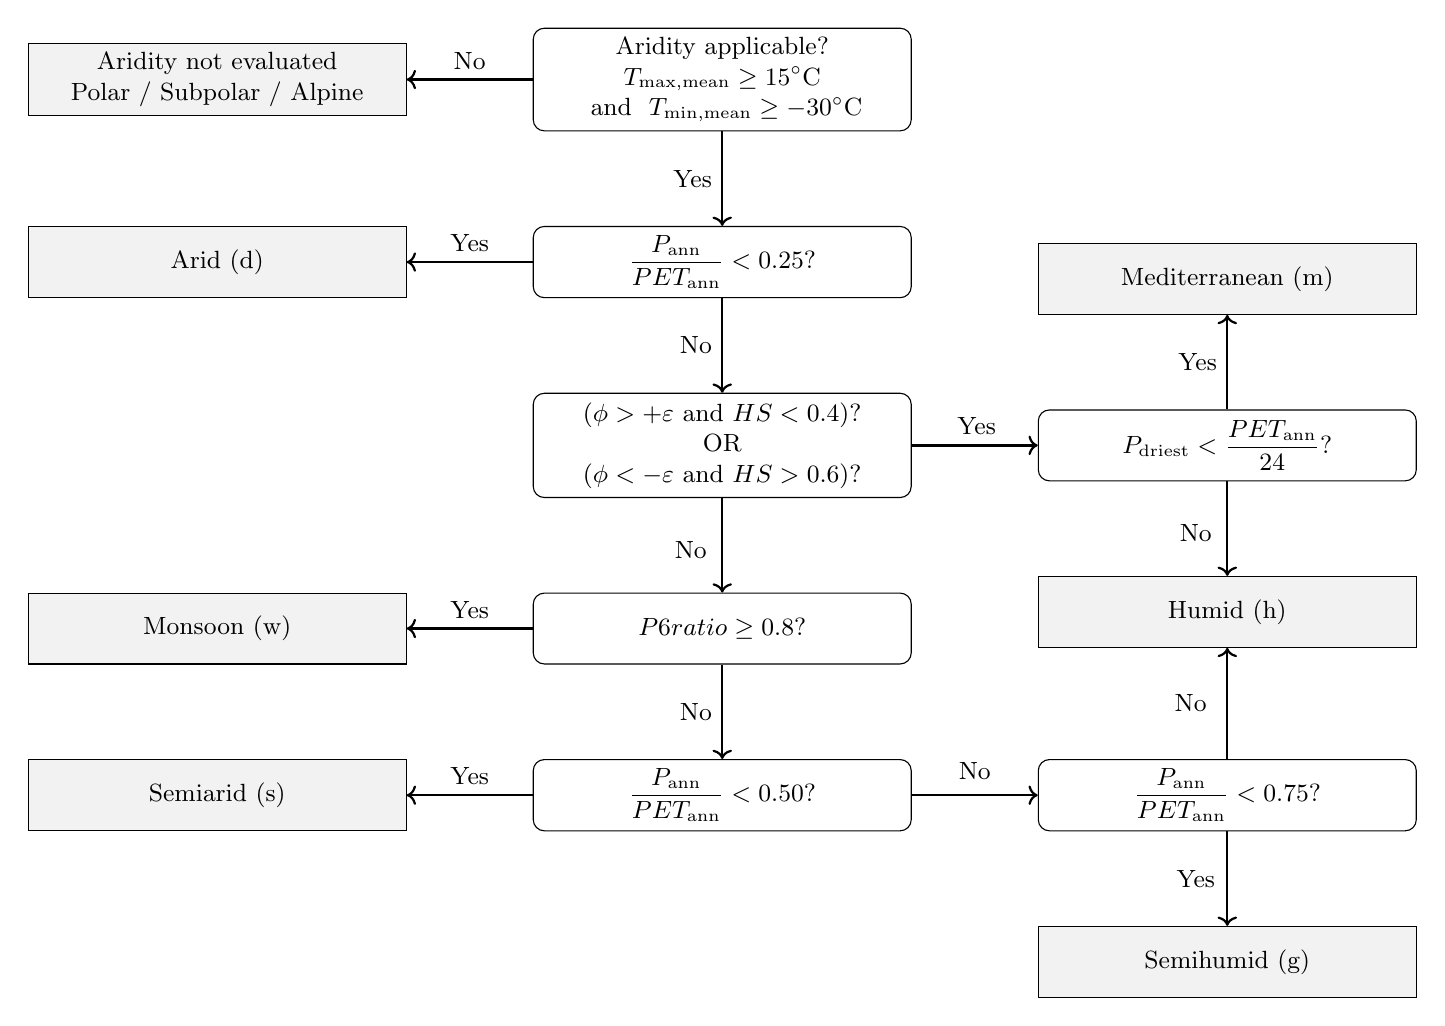
\begin{tikzpicture}[
  node distance=12mm and 16mm,
  decision/.style={
    rectangle, draw, rounded corners,
    align=center, font=\small,
    minimum width=4.8cm, minimum height=9mm
  },
  outcome/.style={
    rectangle, draw,
    align=center, font=\small,
    fill=gray!10,
    minimum width=4.8cm, minimum height=9mm
  },
  arrow/.style={->, thick}
]

% =====================================================
% START
% =====================================================

\node[decision] (relevance)
{Aridity applicable?\\
$T_{\max,\mathrm{mean}} \ge 15^\circ\mathrm{C}$\\
$\text{ and }
\ T_{\min,\mathrm{mean}} \ge -30^\circ\mathrm{C}$};

\node[outcome, left=of relevance] (polar)
{Aridity not evaluated\\
Polar / Subpolar / Alpine};

\draw[arrow] (relevance) -- node[above,font=\small]{No} (polar);

% =====================================================
% ARID CHECK
% =====================================================

\node[decision, below=of relevance] (aridcheck)
{$\dfrac{P_{\mathrm{ann}}}{PET_{\mathrm{ann}}} < 0.25$?};

\node[outcome, left=of aridcheck] (arid)
{Arid (d)};

\draw[arrow] (relevance) -- node[left,font=\small]{Yes} (aridcheck);
\draw[arrow] (aridcheck) -- node[above,font=\small]{Yes} (arid);

% =====================================================
% MEDITERRANEAN CHECK
% =====================================================

\node[decision, below=of aridcheck] (medcheck)
{$(\phi > +\varepsilon \text{ and }
 HS < 0.4)?$\\
$\text{ OR }$\\
$(\phi < -\varepsilon \text{ and }
 HS > 0.6)?$};

\draw[arrow] (aridcheck) -- node[left,font=\small]{No} (medcheck);

\node[decision, right=of medcheck] (medoverride)
{$P_{\text{driest}} < \dfrac{PET_{\text{ann}}}{24}$?};

\node[outcome, below=of medoverride] (humid)
{Humid (h)};

\node[outcome, above=of medoverride] (med)
{Mediterranean (m)};

\draw[arrow] (medcheck) -- node[left,font=\small, xshift=4mm, yshift=2.5mm]{Yes} (medoverride);
\draw[arrow] (medoverride) -- node[above,font=\small, xshift=-4mm, yshift=-3mm]{No} (humid);
\draw[arrow] (medoverride) -- node[left,font=\small]{Yes} (med);

% =====================================================
% MONSOON CHECK
% =====================================================

\node[decision, below=of medcheck] (monsooncheck)
{$P6ratio \ge 0.8$?};

\node[outcome, left=of monsooncheck] (monsoon)
{Monsoon (w)};

\draw[arrow] (medcheck) -- node[above,font=\small, xshift=-4mm, yshift=-3mm]{No} (monsooncheck);
\draw[arrow] (monsooncheck) -- node[above,font=\small]{Yes} (monsoon);

% =====================================================
% HUMIDITY SPLIT
% =====================================================

\node[decision, below=of monsooncheck] (semiaridcheck)
{$\dfrac{P_{\mathrm{ann}}}{PET_{\mathrm{ann}}} < 0.50$?};

\node[outcome, left=of semiaridcheck] (semiarid)
{Semiarid (s)};

\draw[arrow] (monsooncheck) -- node[left,font=\small]{No} (semiaridcheck);
\draw[arrow] (semiaridcheck) -- node[above,font=\small]{Yes} (semiarid);

\node[decision, right=of semiaridcheck] (semihumidcheck)
{$\dfrac{P_{\mathrm{ann}}}{PET_{\mathrm{ann}}} < 0.75$?};

\draw[arrow] (semiaridcheck) -- node[below,font=\small, yshift=5.5mm]{No} (semihumidcheck);

\node[outcome, below=of semihumidcheck] (semihumid)
{Semihumid (g)};

% NOTE: Humid (H) node already exists elsewhere
\draw[arrow] (semihumidcheck) -- node[above,font=\small, xshift=-4mm, yshift=-2.5mm]{Yes} (semihumid);
\draw[arrow] (semihumidcheck) -- node[right,font=\small, xshift=-8mm]{No} (humid);

\end{tikzpicture}
}

\caption{
Decision tree for assigning aridity regimes in the Dickinson
classification.\\\\
\textbf{Note:} $\phi$ denotes geographic latitude in degrees.
Mediterranean seasonality is evaluated only at extratropical locations,
defined as latitudes poleward of the tropics (i.e., exceeding the Earth's axial tilt).
}
\end{figure}

\begin{figure}[htbp]
\centering
\includegraphics[width=\textwidth]{global_aridity_1981-2010.png}
\label{fig:example}
\end{figure}

\begin{figure}[htbp]
\centering
\includegraphics[width=\textwidth]{aridity_legend}
\caption{
Global distribution of aridity zones under the
Dickinson Climate Classification, based on 1981--2010 climatological normals.
Data were processed and plotted in Google Earth Engine (GEE) using
CHELSA BIOCLIM+ v2.1 1981-2010 precipitation and Penman-Monteith PET fields.
}
\label{fig:example}
\end{figure}
\FloatBarrier

% ============================================================
\section{Warm-Month Thermal Zones}

In addition to cold-season thermal constraints, the Dickinson
classification characterizes the intensity of the warm season using the
climatological warmest-month mean near-surface air temperature
($T_{\max,\text{mean}}$). This metric provides a stable measure of summer
thermal conditions that reflects seasonal energy balance rather than
short-lived extreme events.

Warm-month thermal zones are assigned based on $T_{\max,\text{mean}}$ and
are intended to distinguish climates with similar winter conditions but
substantially different summer heat regimes. The resulting categories span
the full range of plausible summer thermal environments, from persistently
cold summers to extreme hyperthermal regimes that may occur under deep-time
or future warming scenarios.

Based on the warmest-month mean temperature, climates are assigned to one
of the following warm-month thermal zones:
\[
\begin{array}{ll}
\text{Hypercaneal Summer (H)}      & T_{\max,\text{mean}} \ge 50^\circ\text{C} \\
\text{Hyperthermal Summer (X)}     & 40 \le T_{\max,\text{mean}} < 50^\circ\text{C} \\
\text{Scorching Summer (z2)}       & 35 \le T_{\max,\text{mean}} < 40^\circ\text{C} \\
\text{Very Hot Summer (z1)}        & 30 \le T_{\max,\text{mean}} < 35^\circ\text{C} \\
\text{Hot Summer (a2)}             & 25 \le T_{\max,\text{mean}} < 30^\circ\text{C} \\
\text{Warm Summer (a1)}            & 20 \le T_{\max,\text{mean}} < 25^\circ\text{C} \\
\text{Cool Summer (b2)}            & 15 \le T_{\max,\text{mean}} < 20^\circ\text{C} \\
\text{Cold Summer (b1)}            & 10 \le T_{\max,\text{mean}} < 15^\circ\text{C} \\
\text{Very Cold Summer (c2)}       & 5 \le T_{\max,\text{mean}} < 10^\circ\text{C} \\
\text{Freezing Summer (c1)}        & 0 \le T_{\max,\text{mean}} < 5^\circ\text{C} \\
\text{Frigid Summer (Y)}           & T_{\max,\text{mean}} < 0^\circ\text{C}
\end{array}
\]

As with the cold-month thermal zones, warm-month thresholds are evenly
spaced in temperature and are intended to represent thermodynamic regimes
rather than biological or impact-based categories. This approach ensures
consistency across paleoclimates, present-day climates, and projected
future warming scenarios without reliance on species-specific tolerance
limits or human comfort thresholds.

\begin{figure}[htbp]
\centering
\includegraphics[width=\textwidth]{global_warm_month_1981-2010.png}
\label{fig:example}
\end{figure}

\begin{figure}[htbp]
\centering
\includegraphics[width=\textwidth]{cold_month_legend}
\caption{
Global distribution of warm-month thermal zones under the
Dickinson Climate Classification, based on 1981--2010 climatological normals.
Data were processed and plotted in Google Earth Engine (GEE) using
CHELSA BIOCLIM+ v2.1 1981-2010 temperature fields.
}
\label{fig:example}
\end{figure}

% ============================================================
\section{Illustrative Complete Climate Codes}

The following examples demonstrate the semantic interpretation of
complete Dickinson climate codes.  
Each code is composed of a cold-month thermal zone, an aridity regime
(where applicable), and a warm-month thermal zone, as defined in the
preceding sections.  
These examples are illustrative only and do not necessarily exist on Earth.

\begin{itemize}
  \item \textbf{YY} —
  Superarctic with frigid summer (aridity not evaluated).

  \item \textbf{Fa2} —
  Subarctic with hot summer (aridity not evaluated).
  
  \item \textbf{Ema1} —
  Continental Mediterranean with warm summer.

  \item \textbf{CdX} —
  Subtropical arid with hyperthermal summer.
  
  \item \textbf{Bb1} —
  Tropical with cold summer (aridity not evaluated).

  \item \textbf{Bhb2} —
  Tropical humid with cool summer.

  \item \textbf{Zgz2} —
  Hyperequatorial semihumid with scorching summer.

\end{itemize}

% ============================================================
\section*{Conclusion}

The Dickinson Comprehensive Climate Classification provides a complete, thermodynamically grounded partition of climate space without imposing biological assumptions or temporal constraints. By formalizing aridity relevance, seasonality diagnostics, and exception handling, the system remains stable under extreme warming, deep-time climates, and hypothetical planetary environments.

% ============================================================
\section*{References}

Brun P., Zimmermann N. E., Hari C., Pellissier L., Karger D. N. (2022).
Global climate-related predictors at kilometre resolution for the past and future.
\textit{Earth System Science Data}, 14, 5573–5603.
https://doi.org/10.5194/essd-14-5573-2022

Emanuel, K. A. (1988).
The maximum intensity of hurricanes.
\textit{Journal of the Atmospheric Sciences}, 45(7), 1143--1155.
https://doi.org/10.1175/1520-0469(1988)045<1143:TMIOH>2.0.CO;2

Karger D.N., Conrad O., Böhner J., Kawohl T., Kreft H., Soria-Auza R.W., Zimmermann N.E., Linder P., Kessler M. (2017).
Climatologies at high resolution for the earth’s land surface areas.
\textit{Scientific Data} 4:170122.
https://doi.org/10.1038/sdata.2017.122

Köppen W. 
Die Wärmezonen der Erde, nach der Dauer der heissen, gemässigten und kalten Zeit und nach der Wirkung der Wärme auf die organische Welt betrachtet.
\textit{Meteorologische Zeitschrift} 1884;1:215–26.

United Nations Environment Programme. (1992).
\textit{World Atlas of Desertification} (2nd ed.).
Edward Arnold, London.

\end{document}
